\subsectionaddtolist{آ}

\[
(a + b)^*a(a + b)^*
\]

ابتدا NFA را برای عبارت منظم داده‌شده رسم می‌کنیم:

\begin{center}
\english
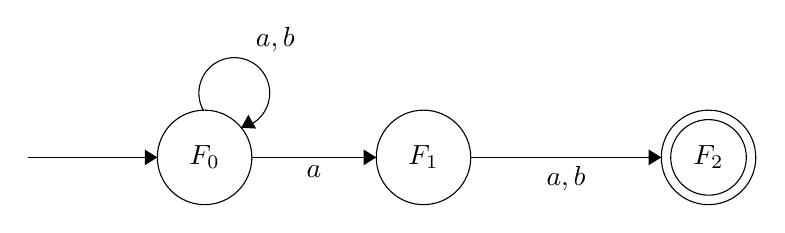
\begin{tikzpicture}[scale=0.2]
\tikzstyle{every node}+=[inner sep=0pt]
\draw [black] (30,-33.2) circle (3);
\draw (30,-33.2) node {$F_1$};
\draw [black] (16.1,-33.2) circle (3);
\draw (16.1,-33.2) node {$F_0$};
\draw [black] (48.1,-33.2) circle (3);
\draw (48.1,-33.2) node {$F_2$};
\draw [black] (48.1,-33.2) circle (2.4);
\draw [black] (4.9,-33.2) -- (13.1,-33.2);
\fill [black] (13.1,-33.2) -- (12.3,-32.7) -- (12.3,-33.7);
\draw [black] (16.022,-30.213) arc (209.22486:-78.77514:2.25);
\draw (20.59,-26.56) node [above] {$a,b$};
\fill [black] (18.42,-31.32) -- (19.37,-31.37) -- (18.88,-30.49);
\draw [black] (19.1,-33.2) -- (27,-33.2);
\fill [black] (27,-33.2) -- (26.2,-32.7) -- (26.2,-33.7);
\draw (23.05,-33.7) node [below] {$a$};
\draw [black] (33,-33.2) -- (45.1,-33.2);
\fill [black] (45.1,-33.2) -- (44.3,-32.7) -- (44.3,-33.7);
\draw (39.05,-33.7) node [below] {$a,b$};
\end{tikzpicture}
\farsi
\end{center}

حال آن را تبدیل به DFA می‌کنیم.
فرض می‌کنیم یک استیت برای حالتی که آخرین حرف $a$
است داریم. یک استیت برای 
$aa$
. یک استیت هم برای 
$ab$
.
اگر آخر عبارت ما $aa$ یا $ab$ داشته باشیم، پس استیت ما یک استیت Final است.


\begin{center}
    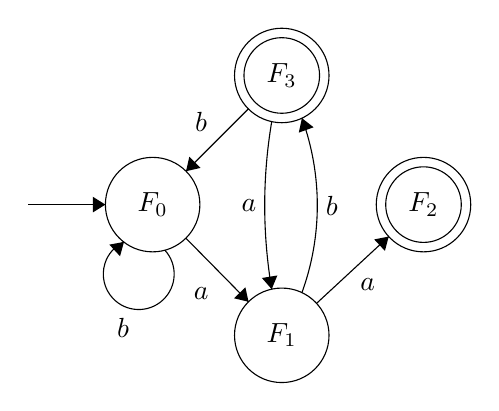
\begin{tikzpicture}[scale=0.2]
    \tikzstyle{every node}+=[inner sep=0pt]
    \draw [black] (15.6,-32.5) circle (3);
    \draw (15.6,-32.5) node {$F_0$};
    \draw [black] (23.8,-40.8) circle (3);
    \draw (23.8,-40.8) node {$F_1$};
    \draw [black] (32.8,-32.5) circle (3);
    \draw (32.8,-32.5) node {$F_2$};
    \draw [black] (32.8,-32.5) circle (2.4);
    \draw [black] (23.8,-24.3) circle (3);
    \draw (23.8,-24.3) node {$F_3$};
    \draw [black] (23.8,-24.3) circle (2.4);
    \draw [black] (7.7,-32.5) -- (12.6,-32.5);
    \fill [black] (12.6,-32.5) -- (11.8,-32) -- (11.8,-33);
    \draw [black] (16.371,-35.387) arc (42.69007:-245.30993:2.25);
    \draw (13.72,-39.71) node [below] {$b$};
    \fill [black] (13.78,-34.87) -- (12.85,-35.04) -- (13.53,-35.78);
    \draw [black] (17.71,-34.63) -- (21.69,-38.67);
    \fill [black] (21.69,-38.67) -- (21.49,-37.75) -- (20.77,-38.45);
    \draw (19.18,-38.12) node [left] {$a$};
    \draw [black] (26.01,-38.77) -- (30.59,-34.53);
    \fill [black] (30.59,-34.53) -- (29.67,-34.71) -- (30.35,-35.44);
    \draw (29.26,-37.14) node [below] {$a$};
    \draw [black] (25.08,-27.009) arc (19.98786:-19.98786:16.211);
    \fill [black] (25.08,-27.01) -- (24.88,-27.93) -- (25.82,-27.59);
    \draw (26.56,-32.55) node [right] {$b$};
    \draw [black] (21.68,-26.42) -- (17.72,-30.38);
    \fill [black] (17.72,-30.38) -- (18.64,-30.17) -- (17.93,-29.46);
    \draw (18.68,-27.92) node [above] {$b$};
    \draw [black] (23.162,-37.87) arc (-170.41227:-189.58773:31.939);
    \fill [black] (23.16,-37.87) -- (23.52,-37) -- (22.54,-37.16);
    \draw (22.22,-32.55) node [left] {$a$};
    \end{tikzpicture}
    \end{center}


\subsectionaddtolist{ب}

\[
(a + b)^*(a+ba)^*a(b+ab)^*
\]

ابتدا NFA را برای عبارت منظم داده‌شده رسم می‌کنیم:

\begin{center}
    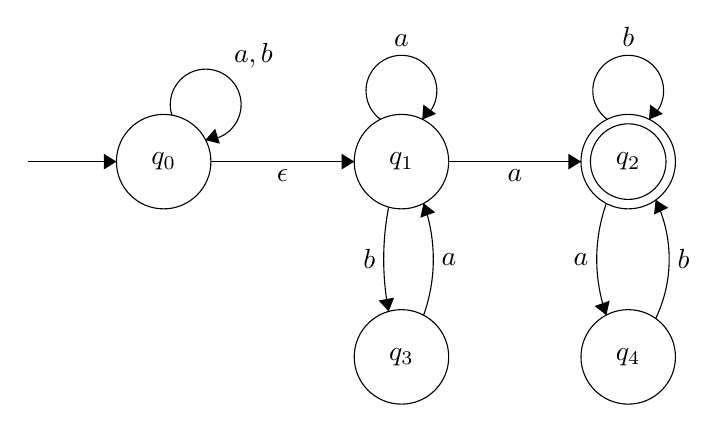
\begin{tikzpicture}[scale=0.2]
    \tikzstyle{every node}+=[inner sep=0pt]
    \draw [black] (13.6,-28.5) circle (3);
    \draw (13.6,-28.5) node {$q_0$};
    \draw [black] (28.7,-28.5) circle (3);
    \draw (28.7,-28.5) node {$q_1$};
    \draw [black] (28.7,-40.9) circle (3);
    \draw (28.7,-40.9) node {$q_3$};
    \draw [black] (43.1,-28.5) circle (3);
    \draw (43.1,-28.5) node {$q_2$};
    \draw [black] (43.1,-28.5) circle (2.4);
    \draw [black] (43.1,-40.9) circle (3);
    \draw (43.1,-40.9) node {$q_4$};
    \draw [black] (5,-28.5) -- (10.6,-28.5);
    \fill [black] (10.6,-28.5) -- (9.8,-28) -- (9.8,-29);
    \draw [black] (14.125,-25.558) arc (197.61565:-90.38435:2.25);
    \draw (19.3,-22.57) node [above] {$a,b$};
    \fill [black] (16.25,-27.13) -- (17.17,-27.36) -- (16.87,-26.41);
    \draw [black] (16.6,-28.5) -- (25.7,-28.5);
    \fill [black] (25.7,-28.5) -- (24.9,-28) -- (24.9,-29);
    \draw (21.15,-29) node [below] {$\epsilon$};
    \draw [black] (27.377,-25.82) arc (234:-54:2.25);
    \draw (28.7,-21.25) node [above] {$a$};
    \fill [black] (30.02,-25.82) -- (30.9,-25.47) -- (30.09,-24.88);
    \draw [black] (27.887,-38.016) arc (-169.13767:-190.86233:17.597);
    \fill [black] (27.89,-38.02) -- (28.23,-37.14) -- (27.25,-37.32);
    \draw (27.07,-34.7) node [left] {$b$};
    \draw [black] (31.7,-28.5) -- (40.1,-28.5);
    \fill [black] (40.1,-28.5) -- (39.3,-28) -- (39.3,-29);
    \draw (35.9,-29) node [below] {$a$};
    \draw [black] (41.777,-25.82) arc (234:-54:2.25);
    \draw (43.1,-21.25) node [above] {$b$};
    \fill [black] (44.42,-25.82) -- (45.3,-25.47) -- (44.49,-24.88);
    \draw [black] (41.712,-38.252) arc (-160.43832:-199.56168:10.608);
    \fill [black] (41.71,-38.25) -- (41.92,-37.33) -- (40.97,-37.67);
    \draw (40.6,-34.7) node [left] {$a$};
    \draw [black] (44.839,-30.927) arc (25.73328:-25.73328:8.691);
    \fill [black] (44.84,-30.93) -- (44.74,-31.86) -- (45.64,-31.43);
    \draw (46.2,-34.7) node [right] {$b$};
    \draw [black] (30.102,-31.141) arc (19.79426:-19.79426:10.511);
    \fill [black] (30.1,-31.14) -- (29.9,-32.06) -- (30.84,-31.72);
    \draw (31.22,-34.7) node [right] {$a$};
    \end{tikzpicture}
    \end{center}

سپس با استفاده از الگوریتم تبدیل NFA به DFA ، DFA آن را به دست می‌آوریم:


\begin{center}
    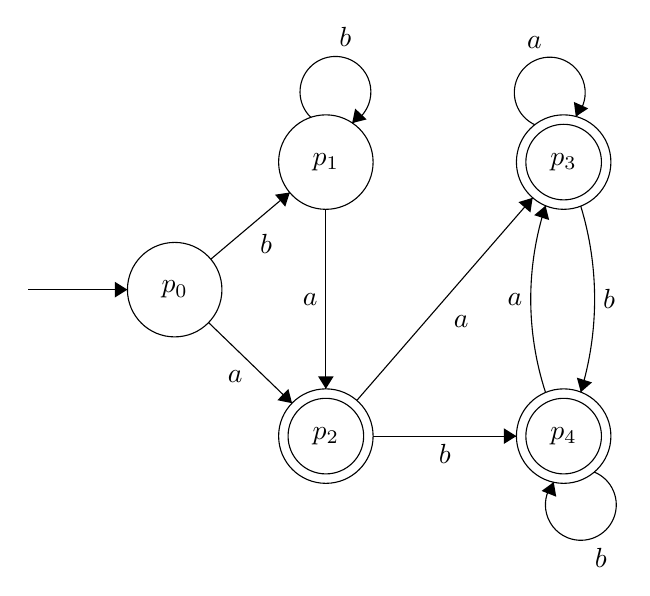
\begin{tikzpicture}[scale=0.2]
    \tikzstyle{every node}+=[inner sep=0pt]
    \draw [black] (14.6,-25.9) circle (3);
    \draw (14.6,-25.9) node {$p_0$};
    \draw [black] (24.2,-17.8) circle (3);
    \draw (24.2,-17.8) node {$p_1$};
    \draw [black] (24.2,-35.2) circle (3);
    \draw (24.2,-35.2) node {$p_2$};
    \draw [black] (24.2,-35.2) circle (2.4);
    \draw [black] (39.3,-17.8) circle (3);
    \draw (39.3,-17.8) node {$p_3$};
    \draw [black] (39.3,-17.8) circle (2.4);
    \draw [black] (39.3,-35.2) circle (3);
    \draw (39.3,-35.2) node {$p_4$};
    \draw [black] (39.3,-35.2) circle (2.4);
    \draw [black] (5.3,-25.9) -- (11.6,-25.9);
    \fill [black] (11.6,-25.9) -- (10.8,-25.4) -- (10.8,-26.4);
    \draw [black] (16.89,-23.97) -- (21.91,-19.73);
    \fill [black] (21.91,-19.73) -- (20.97,-19.87) -- (21.62,-20.63);
    \draw (20.41,-22.34) node [below] {$b$};
    \draw [black] (16.75,-27.99) -- (22.05,-33.11);
    \fill [black] (22.05,-33.11) -- (21.82,-32.2) -- (21.12,-32.92);
    \draw (18.44,-31.03) node [below] {$a$};
    \draw [black] (23.252,-14.966) arc (226.23483:-61.76517:2.25);
    \draw (25.43,-10.52) node [above] {$b$};
    \fill [black] (25.87,-15.32) -- (26.79,-15.09) -- (26.06,-14.4);
    \draw [black] (24.2,-20.8) -- (24.2,-32.2);
    \fill [black] (24.2,-32.2) -- (24.7,-31.4) -- (23.7,-31.4);
    \draw (23.7,-26.5) node [left] {$a$};
    \draw [black] (26.17,-32.93) -- (37.33,-20.07);
    \fill [black] (37.33,-20.07) -- (36.43,-20.34) -- (37.19,-21);
    \draw (32.29,-27.95) node [right] {$a$};
    \draw [black] (27.2,-35.2) -- (36.3,-35.2);
    \fill [black] (36.3,-35.2) -- (35.5,-34.7) -- (35.5,-35.7);
    \draw (31.75,-35.7) node [below] {$b$};
    \draw [black] (41.233,-37.479) arc (68.03624:-219.96376:2.25);
    \draw (41.66,-42.32) node [below] {$b$};
    \fill [black] (38.67,-38.12) -- (37.9,-38.68) -- (38.83,-39.05);
    \draw [black] (38.151,-32.432) arc (-161.95291:-198.04709:19.148);
    \fill [black] (38.15,-20.57) -- (37.43,-21.17) -- (38.38,-21.48);
    \draw (36.71,-26.5) node [left] {$a$};
    \draw [black] (40.385,-20.594) arc (16.9789:-16.9789:20.225);
    \fill [black] (40.39,-32.41) -- (41.1,-31.79) -- (40.14,-31.49);
    \draw (41.77,-26.5) node [right] {$b$};
    \draw [black] (37.478,-15.432) arc (245.30993:-42.69007:2.25);
    \draw (37.45,-10.6) node [above] {$a$};
    \fill [black] (40.07,-14.91) -- (40.86,-14.39) -- (39.95,-13.98);
    \end{tikzpicture}
    \end{center}